% !TeX root = ../note.tex
\section{Разработка программного средства}\label{sec:development}

Разработанное программное обеспечение представляет собой набор сервисов, написанных на языке \csharp, и клиентское приложение, написанное при помощи JavaScript-фреймворка Vue.js.

На рисунке~\ref{fig:general_scheme} изображена схема взаимодействия сервисов программного средства.

\begin{figure}[ht]
    \centering
    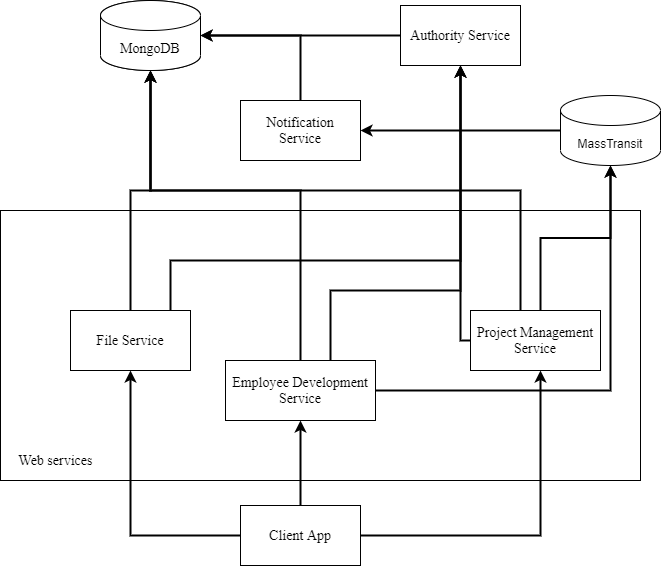
\includegraphics[width=\textwidth]{general_scheme}
    \caption{Схема взаимодействия сервисов}\label{fig:general_scheme}
\end{figure}

В общем виде взаимодействие частей приложения происходит следующим образом:
\begin{itemize}
    \item клиентское приложение используется для того, чтобы работать с необходимой информацией;
    \item в зависимости от вида информации, клиентское приложение отправляет HTTP запросы к сервису развития персонала, сервису управления проектами или файловому сервису;
    \item при необходимости авторизовать действия пользователя данные сервисы отправвляют HTTP запросы к сервису авторизации;
    \item при выполнении необходимых условий сервис развития персонала и сервис управления проектами отправляют события через MassTransit (используется в качестве ``шины''). Очередь данных сообщений обрабатывает сервис уведомлений;
    \item все сервисы используют базу данных для хранения и управления полученными данными.
\end{itemize}

\subsection{Разработка серверной части приложения}\label{sec:development:services}

Серверная часть приложения состоит из следующих .NET сервисов:

\begin{itemize}
    \item employee development service — сервис, который обрабатывает профессиональную информацию пользователей, хранит и обновляет задачи и цели развития;
    \item project management service — сервис, который хранит и обрабатывает информацию о проектах;
    \item file service — сервис, который используется для загрузки и получения пользовательских файлов;
    \item notification service — сервис, который обрабатывает события об отправке уведомлений пользователям;
    \item authority service — сервис, который отвечает за хранение идентификационных данных пользователей и их аутентификацию и авторизацию.
\end{itemize}

Все сервисы, кроме сервиса уведомлений представляют собой ASP.NET Web API приложения, которые обрабатывают HTTP запросы в зависимости от своего назначения. Каждый из этих сервисов имеет адрес ''/api/heartbeat'', который возвращает дату и время на момент запроса и используется для проверки текущего состояния сервиса. Успешный ответ от сервиса по данному адресу означает, что он успешно запущен и может обрабатывать запросы.

Все сервисы разбиты на множество проектов, которые можно выделить в следующие группы:

\begin{itemize}
    \item domain model - проекты, которые содержат классы, используемые в БД;
    \item repository - проекты, которые содержат функционал для обмена информацией с БД при помощи классов доменной модели;
    \item foundation — проекты, который содержат специфическую бизнес-логику сервисов;
    \item views - проекты, которые являются проверяют полученные от пользователей данные и передают их в проекты бизнес-логики для обработки.
\end{itemize}

Проекты группы domain model являются общими для всех сервисов. Они содержат простые классы .NET, которые представляют собой проекции коллекций базы данных MongoDB на приложение. Большинство из них наследуют интерфейс ''IMongoEntity'', что позволяет определять имя MongoDB коллекции, однако возможно использование и обычных классов. В таком случае имя коллекции будет названием класса взятом в множественном числе и написанное в ''змеином'' регистре.

Проекты группы repository также являются общими для всех сервисов. Они содержат функционал для обмена информацией с БД. В них определены интерфейсы ''IRepository'' и ''IUnitOfWork'', которые соответствуют паттернам программирования ''Репозиторий'' и ''Единица работы''.

Паттерн ''Репозиторий'' - это слой абстракции, инкапсулирующий в себе всё, что относится к способу хранения данных. Его назначение - разделение бизнес-логики от деталей реализации слоя доступа к данным.

Паттерн ''Единица работы'' используется для гарантии атомарности обращений к БД в рамках бизнес-логики. Это означает, что любая операция бизнес-логики может совершать сколько угодно обращений к БД, однако её изменение будет проводиться одной транзакцией, что позволит избежать проблем с параллельным изменением одного и того же объекта, а также позволит отменить все изменения, если какое-то завершилось с ошибкой.

На рисунке~\ref{fig:repo_classes} приведена диаграмма классов проекта «DataAccess», который является проектом группы repository и содержит реализации паттернов ''Репозиторий'' и ''Единица работы''. 

\begin{figure}[ht]
    \centering
    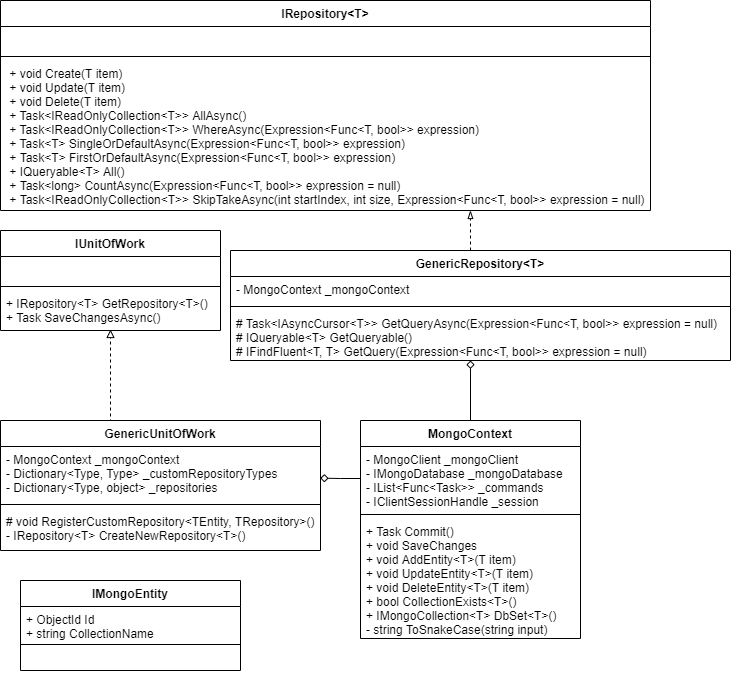
\includegraphics[width=\textwidth]{repo_classes}
    \caption{Диаграмма классов проекта «DataAccess»}\label{fig:repo_classes}
\end{figure}

\bigskip
\textbf{Сервис развития персонала}

Сервис развития персонала используется для сценариев, связанных с развитием сотрудников. Он позволяет экономить время менеджеров, увеличивать их продуктивность, а также улучшает прозрачность некоторых взаимоотношений в организации.

Среди сценариев использования сервиса можно выделить создание профилей для новых сотрудников и менеджеров, обновление информации о пользователях и технологиях. С помощью данного сотрудники могут сдавать мини-экзамены своим более опытным коллегам, что положительно сказывается на их профессиональных навыках. В общем виде алгоритм такого экзамена следующий:

\begin{itemize}
    \item Сотрудник договаривается с коллегой о деталях экзамена.
    \item Сервис создаёт запись в БД с полной информацией, а также создаёт сообщение в очереди MassTransit для сервиса уведомлений.
    \item Сотрудники проводят мини-экзамен, и на основе результатов экзаменатор обновляет статус (сдан или нет).
    \item Сервис обновляет запись в БД и снова создаёт сообщение в очереди MassTransit для сервиса уведомлений.
\end{itemize}

На рисунке~\ref{fig:pass_exam_diagram} приведена диаграмма последовательности «сдача мини-экзамена». 

\begin{figure}[ht]
    \centering
    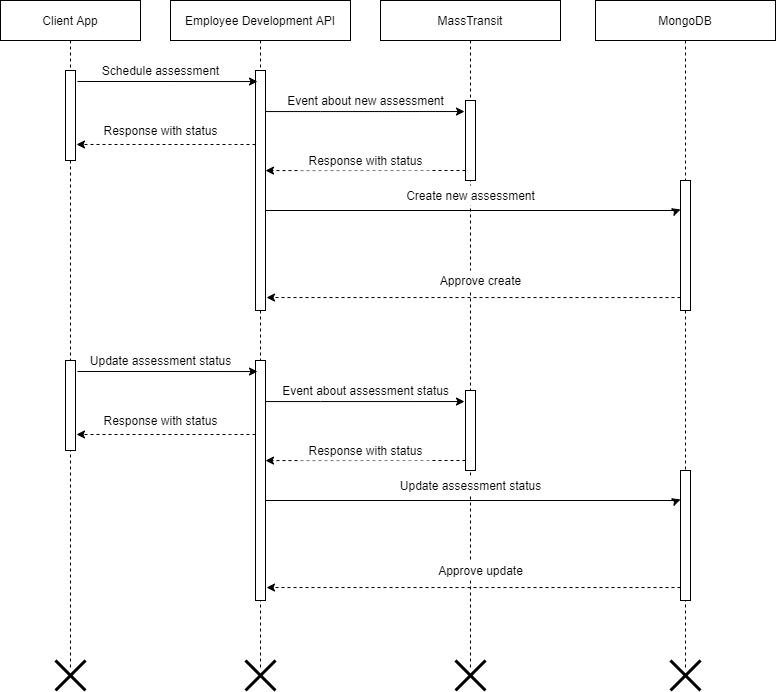
\includegraphics[width=\textwidth]{pass_exam_diagram}
    \caption{Диаграмма последовательности «сдача мини-экзамена»}\label{fig:pass_exam_diagram}
\end{figure}

Данный сервис представляет собой ASP.NET Web API приложение, которое обрабатывает HTTP запросы, связанные с развитием сотрудников. Среди .NET контроллеров, которые обрабатывают запросы, можно выделить следующие:

\begin{itemize}
    \item developed employees controller - используется для работы с информацией о сотруднике;
    \item skills controller - используется для работы с информацией о технологиях в компании;
    \item assessments controller - используется для информации о мини-экза\-менах между сотрудниками.
\end{itemize}

\bigskip
\textbf{Сервис управления проектами}

Сервис управления проектами используется для работы с информацией о проектах и текущих задачах внутри них.

Данный сервис представляет собой ASP.NET Web API приложение, которое обрабатывает HTTP запросы, связанные с проектами компании и задачах в этих проектах. Среди .NET контроллеров, которые обрабатывают запросы, можно выделить следующие:

\begin{itemize}
    \item projects controller - используется для работы с информацией о проектах в компании;
    \item tasks controller - используется для работы с информацией о текущих задачах в проектах компании.
\end{itemize}

\bigskip
\textbf{Файловый сервис}

Файловый сервис используется для загрузки и получения пользовательских файлов.

Данный сервис представляет собой ASP.NET Web API приложение, которое обрабатывает HTTP запросы, связанные с пользовательскими файлами. Сервис имеет следующий интерфейс:

\begin{itemize}
    \item получить загруженный файл по его идентификатору;
    \item загрузить новый файл.
\end{itemize}

Все файлы загруженные пользователями файлы хранятся в Firebase хранилище. Пример загруженных файлов приведён на рисунке~\ref{fig:firebase_files}. Выбор в пользу такого метода хранения был сделан на основе оценки сочетания объема доступного дискового пространства, цены и скорости работы.

\begin{figure}[ht]
    \centering
    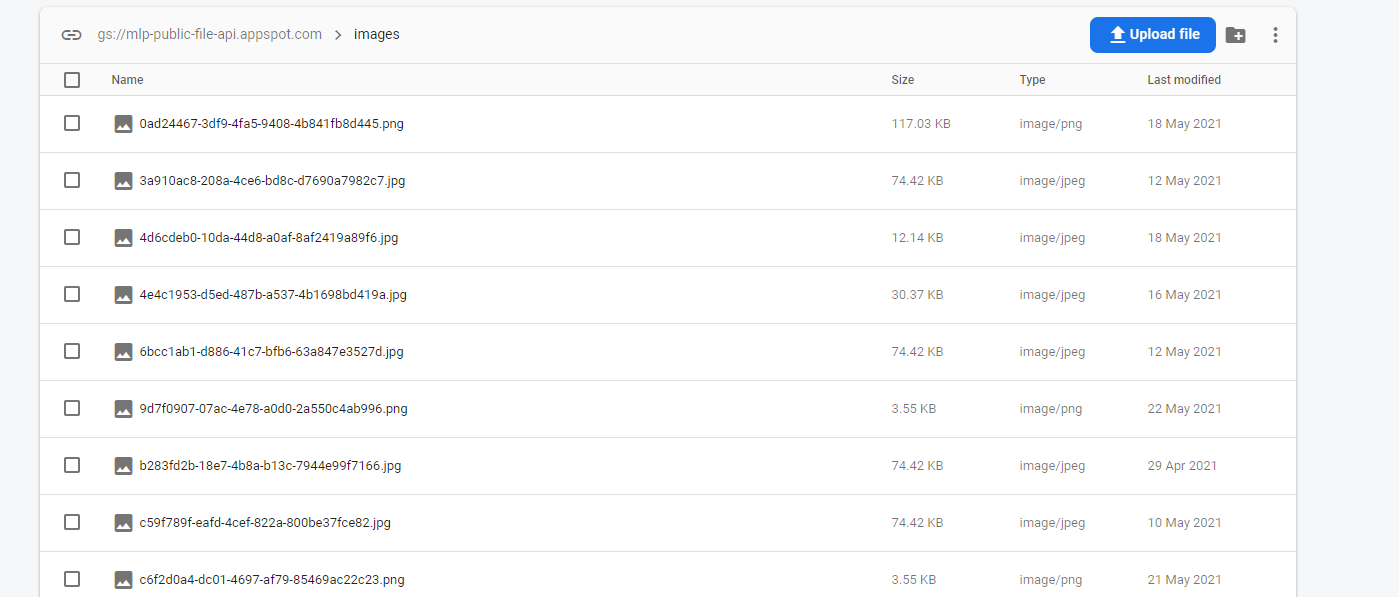
\includegraphics[width=\textwidth]{firebase_files}
    \caption{Пример файлов хранящихся в Firebase хранилище}\label{fig:firebase_files}
\end{figure}

Сервис содержит всего два контроллера, которые обрабатывают HTTP запросы:
\begin{itemize}
    \item genders controller - позволяет загружать любые файлы, которые будут использоваться в качестве гендеров пользователей, объёмом до пяти мегабайт.
    \item images controller - позволяет загружать изображения, которые будут использоваться в качестве фотографий сотрудников, логотипов организации и т.д., объёмом также до пяти мегабайт и в форматах jpeg, png, bmp, tiff.
\end{itemize}

Такое разделение позволяет наложить разные ограничения на файлы гендеров и изображений.

\bigskip
\textbf{Сервис уведомлений}

Сервис уведомлений используется для того, чтобы оповещать менеджеров и сотрудников о всех события в организации, которые они должны знать.

Данный сервис представляет собой .NET приложение, которое обрабатывает очередь сообщений RabbitMQ. Сервис формирует уведомление на основе поступающих сообщений и шаблонов, загруженных в БД. После того, как шаблон успешно сформирован, уведомление отправляется пользователю на электронную почту указанную при регистрации. Пример такого уведомления приведён на рисунке~\ref{fig:email_example}.

\begin{figure}[ht]
    \centering
    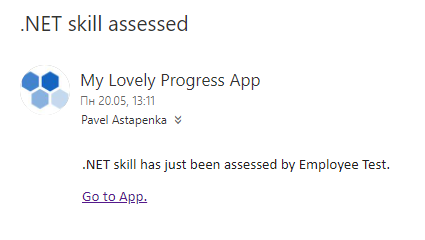
\includegraphics[width=\textwidth]{email_example}
    \caption{Пример отправляемого пользователю уведомления}\label{fig:email_example}
\end{figure}

Для формирования сообщений на основе шаблонов используется бесплатный пакет DotLiquid. Он является портом аналогичного пакета для языка программирования Ruby, характеризуется высокой производительностью и удобным языком разметки, который используется в ряде платформ, например, Node и Python. Он используется для следующих целей:
\begin{itemize}
    \item отделить бизнес-логику и логику шаблонов;
    \item получить возможность создавать сообщения на основе шаблонов, полученных напрямую из БД;
    \item использовать язык разметки, который существует также для других платформ.
\end{itemize}

Формирование и отправка уведомления происходит следующим образом:
\begin{itemize}
    \item сервис получает из очереди сообщений информацию о новом уведомлении;
    \item из базы данных загружается шаблон уведомления;
    \item сервис при помощи DotLiquid заполняет данные в шаблоне;
    \item сервис отправляет сформированное уведомление по адресу, полученному из сообщения.
\end{itemize}

\bigskip
\textbf{Сервис авторизации}

Сервис авторизации используется для аутентификации и авторизации пользователей. Авторизация происходит следующим образом:

\begin{enumerate}
    \item Отправляется HTTP запрос на получение пары токенов при помощи логина и пароля пользователя.
    \item Access токен из полученной пары указывается в заголовке всех запросов, которые требуют авторизацию. Refresh токен сохраняется.
    \item Когда срок действия access токена истекает, используется refresh токен для получения новой пары.
    \item Если по каким-либо причинам вместе с access токеном стал невалидным refresh токен, то необходимо снова получить пару токенов при логина и пароля пользователя.
\end{enumerate}

Access и refresh токены представляют собой JWT токены, которые содержат в себе всю необходимую информацию об авторизованном пользователе.

JSON Web Token (JWT) — это открытый стандарт (RFC 7519)~\cite{jwt} для создания токенов доступа, основанный на формате JSON. Как правило, используется для передачи данных для аутентификации в клиент-серверных приложениях. Токены создаются сервером, подписываются секретным ключом и передаются клиенту, который в дальнейшем использует данный токен для подтверждения своей личности.

Токен JWT состоит из трех частей: заголовка (header), полезной нагрузки (payload) и подписи или данных шифрования. Первые два элемента — это JSON объекты определенной структуры. Третий элемент вычисляется на основании первых и зависит от выбранного алгоритма (в случае использования не подписанного JWT может быть опущен). Токены могут быть перекодированы в компактное представление (JWS/JWE Compact Serialization): к заголовку и полезной нагрузке применяется алгоритм кодирования Base64-URL, после чего добавляется подпись и все три элемента разделяются точками (``.'').

К примеру, для заголовка и полезной нагрузки, которые выглядят следующим образом:

\begin{lstlisting}[language=javascript]
{
  "alg": "HS512",
  "typ": "JWT"
}
{
  "sub": "12345",
  "name": "John Gold",
  "admin": true
}
\end{lstlisting}

Получим следующее компактное представление (переводы строки добавлены для наглядности):

\begin{lstlisting}
eyJhbGciOiJIUzUxMiIsInR5cCI6IkpXVCJ9.
eyJzdWIiOiIxMjM0NSIsIm5hbWUiOiJKb2hu
IEdvbGQiLCJhZG1pbiI6dHJ1ZX0K.
LIHjWCBORSWMEibq-tnT8ue\_deUqZx1K0XxCOXZRrBI
\end{lstlisting}

Сервис использует следующий интерфейс:

\begin{itemize}
    \item \lstinline{GetTokensByCredentials(login string, password string) : TokenPair, error} — аутентификация существующего пользователя по логину и паролю. Данная операция возвращает пару access и refresh токенов;
    \item \lstinline{GetTokensByRefreshToken(refresh_token string) : TokenPair, error} — ау\-тентификация существующего пользователя по refresh токену. Данная операция возвращает пару access и refresh токенов.
\end{itemize}

В сервисе определены следующие сущности:

\begin{itemize}
    \item Клиент.
    \item Ресурс.
    \item Область видимости.
\end{itemize}

Клиент представляет собой приложение, которое может запрашивать токены у авториационного сервиса. В базе данных определён только один клиент, который используется Vue.js приложением.

Ресурс - защищенная информация, доступ к которой обеспечивает авторизационный сервис. Она может быть как информацией о пользователях, так и API. Каждый ресурс имеет уникальное имя, и клиент обязан использовать его при отправке HTTP запроса, чтобы указать к каким службам он хочет получить доступ.

Область видимости позволяет ограничивать доступ различных клиентов к частям API. Токены доступа, возвращенные сервисом, будут обеспечивать доступ только к тем службам, которые входят в определённую область.

Благодаря данным сущностям в авторизационном сервисе задана схема авторизации ''Resource Owner Password Credentials''. Эта схема очень удобна для программного средства, так как позволяет получить доступ к сервисам используя только логин и пароль пользователя и поддерживает сценарий их интерактивного ввода.

\subsection{Разработка клиентского приложения}\label{sec:development:client_app}

Клиентское приложение определяет базовые обёртки обычных html элементов. Данные компоненты используются во всём приложении для выполнения несложных операций.

Первым таким компонентом является обычная кнопка – «AppButton». Пример такой кнопки представлен на рисунке~\ref{fig:app_button}. Она включает в себя всего один параметр: «disabled». Он определяет, должна ли реагировать кнопка на нажатия. Также он меняет её визуальное состояние, чтобы выделить те кнопки, с которыми нельзя взаимодействовать. При нажатии на кнопку в родительский компонент отправится событие «input».

\begin{figure}[h]
    \centering
    
\includegraphics[width=\textwidth]{app_button}
    \caption{Пример активного AppButton на странице}\label{fig:app_button}
\end{figure}

Следующий базовый компонент – «AppInput». Он представляет собой стилизованное текстовое поле для ввода пользовательских данных. Пример такого компонента представлен на рисунке~\ref{fig:app_input}. Его параметры:

\begin{itemize}
    \item modelValue – текущее значение текстового поля. Оно изменяется при вводе данных пользователем;
    \item тип текстового поля. Работает аналогична с html тегом «input»;
    \item invalid – логическое значение, которое в зависимости от своего значения устанавливает красную границу вокруг поля, указывающую пользователю, что данные введены неверно;
    \item placeholder – текстовое значение появляющееся при пустом вводе.
\end{itemize}

\begin{figure}[h]
    \centering
    
\includegraphics[width=\textwidth]{app_input}
    \caption{Пример AppInput на странице}\label{fig:app_input}
\end{figure}

Для загрузки пользовательского файла используется компонент \\«AppDropbox» (рисунок~\ref{fig:app_dropbox}). При загрузке файла пользователем данный компонент отправляет в родительский компонент событие «input».

\begin{figure}[h]
    \centering
    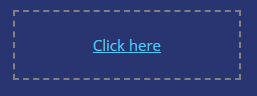
\includegraphics[width=\textwidth]{app_dropbox}
    \caption{Пример AppDropbox на странице}\label{fig:app_dropbox}
\end{figure}

Компонент «AppRadioButton» представляет собой переключатель, который позволяет пользователю выбрать одну опцию из предопределенного набора. Пример такого набора представлен на рисунке~\ref{fig:app_radio_buttons}.

\begin{figure}[h]
    \centering
    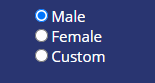
\includegraphics[width=\textwidth]{app_radio_buttons}
    \caption{Пример AppRadioButton на странице}\label{fig:app_radio_buttons}
\end{figure}

Также существует компонент «AppHeader», который используется только один раз в рамках одной страницы. Он задаёт заголовок всего сайта (рисунок~\ref{fig:app_header}). Важно отметить, что содержимое заголовка может изменяться в зависимости от статуса текущего пользователя.

\begin{figure}[h]
    \centering
    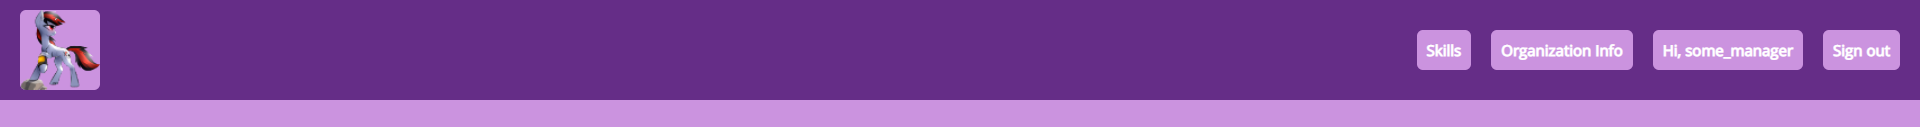
\includegraphics[width=\textwidth]{app_header}
    \caption{Пример компонента AppHeader}\label{fig:app_header}
\end{figure}

Сайт для взаимодействия с пользователем использует только английский язык. Однако вводимые пользователем данные не ограничены использованием только анлийского языка и могут быть на русском, белорусском и т.д.

Рассмотрим vuex-модуль для проекта. Он интегрируется в проект и доступен из любого компонента. В нем содержится информация о текущем пользователе и статусе загрузки страницы. Единственный action модуля заключается в том, чтобы запросить информацию о текущем пользователе с сервера и сохранить её в своём состоянии с помощью мутации.

В модуле имеется 2 мутации:

\begin{itemize}
    \item SET\_USER\_INFO – устанавливает информацию о пользователе при помощи дешифрования JWT токена, полученного от сервиса авторизации;
    \item SET\_LOADING – устанавливает текущее состояние загрузки: страница загружается или не загружается.
\end{itemize}

За все обращения к серверу отвечает файл «api.js». Он представляет собой обертку над библиотекой «axios». Модуль содержит объединенный по категориям список HTTP запросов, с описанными к ним параметрами. Также в этом файле настраивается добавление аутентификационного токена к запросам, что позволяет пользователю не вводить свои логин и пароль неограниченно долго. 

Файл «router.js» отвечает за сопоставление URL к компонентам, которые должны будут использоваться. Одним из основных принципов работы этого модуля является тот факт, что компоненты могут вкладываться друг в друга с помощью тега «router-view» внутри template. Файл включает в себя проверки авторизационных политик, которые определяют ограничения на доступ к компонентам в зависимости от статуса пользователя.

Создается один общий компонент – MainLayout, содержащий базовую общую разметку сайта. В зависимости от содержимого URL, в router-view данного компонента будут попадать разные страницы. Они также могут иметь собственные router-view в зависимости от содержимого URL.

Самые сложные компоненты приложения располагаются в папке «views» (рисунок~\ref{fig:app_view}). Они все имеют сложную разметку, часто применяют внутри себя множество других компонентов, используют уникальные стили, правила валидации и т.д. Большинство данных компонентов служат страницей, на которую ведет URL, однако есть и исключения.

\begin{figure}[h]
    \centering
    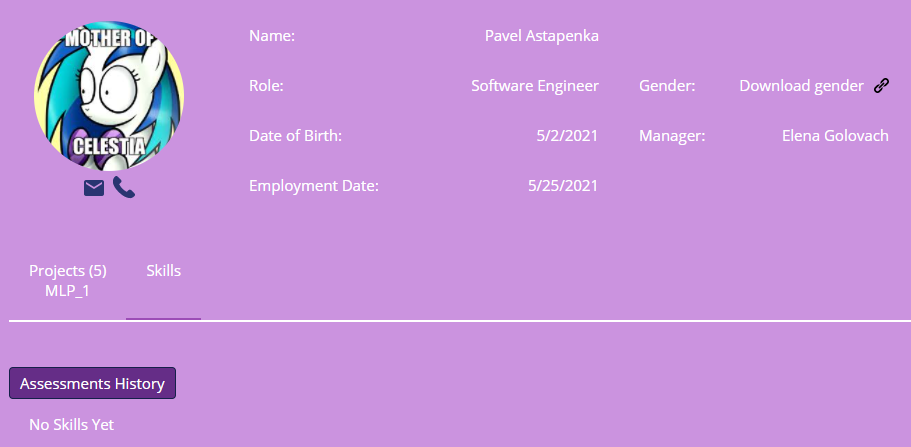
\includegraphics[width=\textwidth]{app_view}
    \caption{Часть страницы UserProfile}\label{fig:app_view}
\end{figure}

Таким образом, разработаны все сервисы необходимые для функционирования программного средства. Создано клиентское приложение, которое предоставляет пользователям быстрый и удобный интерфейс взаимодействия с программным средством.
